%clase del documento
\documentclass[a4paper,12pt]{article}

%paquete de idioma y codificación de caracteres
\usepackage[spanish]{babel}
\usepackage[utf8]{inputenc}
\usepackage{afterpage}

\usepackage{cite} % para contraer referencias
\usepackage{fancyhdr} % para encabezados y pie de pagina

% soporte gráfico
\usepackage{graphicx} % figuras
\usepackage{subfigure} % subfiguras
\graphicspath{ {images/} }

%datos del documento
\author{Ignacio Agüero Salcines}
\title{Especificación Gráfica de Procesos de Recuperación de Datos en LUCA}

\setcounter{tocdepth}{5}
\setcounter{secnumdepth}{5}


% encabezados
\lhead[\thepage]{CAPÍTULO \thechapter. \rightmark}
\chead[]{}
\rhead[CAPÍTULO \thechapter. \leftmark]{\thepage}
\renewcommand{\headrulewidth}{0.5pt}

% pie de pagina
\lfoot[]{\today}
\cfoot[]{}
\rfoot[Ignacio Agüero]{}
\renewcommand{\footrulewidth}{0pt}

% primera pagina de un capitulo
\fancypagestyle{plain}{
	\fancyhead[L]{}
	\fancyhead[C]{}
	\fancyhead[R]{\thepage}
	\fancyfoot[L]{}
	\fancyfoot[C]{}
	\fancyfoot[R]{}
	\renewcommand{\headrulewidth}{0pt}
	\renewcommand{\footrulewidth}{0pt}
}

\pagestyle{fancy}


\begin{document}
	
	\lhead[\thepage]{CAPÍTULO \thechapter. \rightmark}
	\rhead[CAPÍTULO \thechapter. \leftmark]{\thepage}
	
	\pagestyle{empty}
	\tableofcontents
	\cleardoublepage
	
	\pagestyle{plain}
	
	\listoffigures
	\listoftables
	\thispagestyle{empty}
	\cleardoublepage
	
	\pagenumbering{roman}
	\section*{Agradecimientos}
	Me gustaría dar agradecimientos a mi familia y facultad, ya que sin ellos esto no habría sido posible nada de estos.
	
	\vspace{5mm}
	
	\noindent Es importante agradecer también a CIC Consulting Informático por permitirme la oportunidad de realizar el desarrollo del proyecto en su empresa, sin olvidarme de mis compañeros de LUCA, que han sido un gran apoyo durante el mismo..
	
	\vspace{5mm}
	
	\noindent Para finalizar, me gustaría gradecer a mi mentor Pablo, por guiarme durante el desarrollo del proyecto con eficacia y ayudarme a afrontar este trabajo de fin de grado.
	\cleardoublepage
	
	\afterpage{\null\newpage}
	\newpage
	
	
	\section*{Resumen}
	Las empresas actuales utilizan ya no un único sistema de información que de	soporte a sus procesos de trabajo, sino un  ecosistema de sistemas información que dan soporte a diferentes procesos de negocio ejecutados dentro de dicha organización. Como consecuencia de esta nueva situación, cuando un usuario	quiere obtener una información concreta cuyos datos residen en varios de estos
	sistemas, necesita acceder a cada uno de estos sistemas, extraer de cada sistema la información que precisa, filtrarla y unificarla para finalmente	obtener los datos requeridos.
	
	\vspace{5mm}
	
	Por ejemplo, una tienda de electrodomésticos podría tener sistemas informáticos diferentes para el departamento de atención al cliente, para el departamento técnico de postventa y para el departamento de compras y adquisiciones.Por tanto, para conocer el estado actual de una reparación, podríamos necesitar:
		\begin{itemize}
			\item  Acceder al primer sistema para obtener el identificador de la incidencia y en qué fase de su gestión se encuentra.
			\item  Comprobado que la incidencia está actualmente en reparación, recuperaríamos otro sistema el estado detallado de la reparación, comprobando que está a la espera de una pieza.
			\item Finalmente accederíamos al sistema de compra y adquisiciones para comprobar cuando está prevista la entrega de dicha pieza. Los sistemas de almacenamiento de la información puede ser diversos, incluyendo desde un servicio web, una base de datos relacional, un repositorio de ficheros accesible vía FTP o una base de datos NoSQL.
		\end{itemize}
	
	\vspace{5mm}
	
	El objetivo de este proyecto es facilitar dicho proceso de composición al usuario mediante el desarrollo de un mecanismo gráfico para la especificación de estos procesos de composición de consultas.
	

	\vspace{5mm}
	
	\textbf{Palabras clave}: 
	\cleardoublepage
	
	\afterpage{\null\newpage}
	\newpage
	
	\section*{Preface}

	

	\textbf{Keywords}:
	\cleardoublepage
	
	\pagenumbering{arabic}
	\setcounter{page}{1}
	
	\afterpage{\null\newpage}
	\newpage
	
	\section{Introducción}
	
	
	
	En los últimos años, el volumen de datos que una empresa o entidad necesita y/o es capaz de gestionar o manipular, ha aumentado de forma vertiginosa. Además del volumen de datos a manipular, nos damos cuenta de que para acceder a lo diversos datos es necesario muchas veces establecer comunicaciones con los diversos recursos existentes para alcanzar el objetivo.
	
	\vspace{5mm}
	
	
	 Con el objeto de facilitar este proceso de recuperación de información almecenada en sistemas y fuentes de datos hetereogéneas, dentro de la empresa	CIC, se está desarrollando una aplicación denominada LUCA. Para	facilitar este proceso de recuperación de información, LUCA proporciona un lenguaje común para todas las fuentes de datos a unificar, permitiendo al
	usuario abstraerse de los detalles de cada fuente.
	
	\vspace{5mm}
	
	 Actualmente LUCA proporciona mecanismos o abstracciones para permitir al	usuario recuperar de manera uniforme información de diferentes fuentes de datos.	Utilizando el ejemplo anterior, LUCA actualmente propociona mecanismos para
	recuperar información, de la misma forma y mediante las mismas primitivas, de los tres sistemas previamente descritos, aunque sus sistemas de almacenamiento sean radicalmente diferentes.
	
	\vspace{5mm}
	
	 No obstante, LUCA actualmente sólo es capaz recuperar información de una única fuente de datos a la vez. Por tanto, cuando es necesario combinar información procedente de distintas fuentes, tal como ocurre en el ejemplo descrito, el propio usuario es el que debe realizar dicho	proceso de composición, ejecutando cada consulta a mano, y utilizando las salidas de cada una de ellas como las entradas de las siguientes.
	 
	 \vspace{5mm}
	 
	 El objetivo de este proyecto es facilitar dicho proceso de composición al usuario mediante el desarrollo de un mecanismo gráfico para la especificación de estos procesos de composición de consultas.
	 
	 \vspace{5mm}
	 
	 Dado que la empresa solicita que este editor gráfico sea utilizable vía web, se desarrollará utilizando la librería gráfica Javscript Go.JS y el framework Vaadin.
	 
	 	\subsection{Planificación del proyecto}
	 
	 
		\subsection{Estructura del documento}
	 
	  \afterpage{\null\newpage}
	 \newpage
	 
	
	
	\section{Ingeniería de Requisitos}
	
	\afterpage{\null\newpage}
	\newpage
	

	 \section{Análisis y documentación}
	 
	 	\subsection{GO.JS}
	 		
	 		
	 		\begin{figure}[h]
	 			\centering
	 			
\includegraphics[scale=1]{gojs.jpeg}
	 			\caption{GO.JS Logo}\label{fig:gojs}
	 		\end{figure}
	 	
	 	
	 		\subsubsection{¿Qué es GO.JS?}
	 			Go.JS \cite{gojs} es una biblioteca de JavaScript con múltiples funciones para implementar diagramas interactivos personalizados y visualizaciones complejas en navegadores y plataformas web modernos.
	 	
	 		\subsubsection{¿Porqué GO.JS?}
	 		 GoJS facilita la construcción de diagramas de JavaScript de nodos, enlaces y grupos complejos con plantillas y diseños personalizables.
	 		
	 		
	 		\subsubsection{Características}
	 		GoJS ofrece muchas características avanzadas para la interactividad del usuario, tales como arrastrar y soltar, copiar y pegar, edición de texto en el lugar, información sobre herramientas, menús contextuales, diseños automáticos, plantillas, vinculación y modelos de datos, administración de estado transaccional y deshacer, paletas , vistas generales, controladores de eventos, comandos y un sistema de herramientas extensible para operaciones personalizadas.
	 		
	 	
	 		\subsubsection{Explicación}
	 		GoJS ofrece muchas características avanzadas para la interactividad del usuario, tales como arrastrar y soltar, copiar y pegar, edición de texto en el lugar, información sobre herramientas, menús contextuales, diseños automáticos, plantillas, vinculación y modelos de datos, administración de estado transaccional y deshacer, paletas , vistas generales, controladores de eventos, comandos y un sistema de herramientas extensible para operaciones personalizadas.
	 
	 
	 	\subsection{Vaadin}
	 	
	 		\begin{figure}[h]
	 			\centering
	 			
\includegraphics[scale=1]{Vaadin-logo.png}
	 			\caption{Vaadin Logo}\label{fig:Vaadin-logo}
	 		\end{figure}
 		
 			\subsubsection{¿Qué es GO.JS?}
 				Vaadin\cite{vaadin} es un framework de desarrollo de SPA que permite escribir el código de dichas aplicaciones en Java o en cualquier otro lenguaje soportado por la JVM 1.6+. Esto permite la programación de la interfaz gráfica en lenguajes como Java 8, Scala o Groovy, por ejemplo.
 			
 			\subsubsection{Características}
 				Uno de las características diferenciadores de Vaadin es que, contrario a las librerías y frameworks de JavaScript típicas, presenta una arquitectura centrada en el servidor, lo que implica que la mayoría de la lógica es ejecutada en los servidores remotos. Del lado del cliente, Vaadin está construido encima de Google Web Toolkit, con el que puede extenderse.
 	
 			\subsubsection{Aplicación}
 				En este proyecto, Vaadin se encargara de realizar la comunicación entre el cliente y el servidor. De esta forma, será capaz de enviar y recibir datos, eventos y peticiones entre el componente Javascript (cliente) y el servidor.
 			
 			
	 			\begin{figure}[h]
	 				\centering
	 				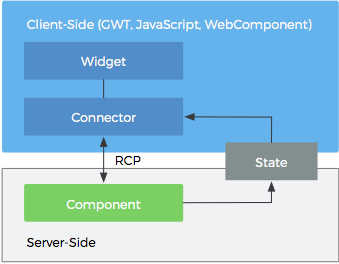
\includegraphics[scale=1.5]{schema.png}
	 				\caption{Esquema Cliente-Servidor}\label{fig:schema}
	 			\end{figure}
 			
 		
	
	\afterpage{\null\newpage}
	\newpage
	
	\section{Diseño Arquitectónico}
	
	El diseño arquitectónico va a describir tanto la estructura arquitectónica del componente de procesos implementado con GO.js, tanto su integración en el producto LUCA, el cual, requiere de un diseño paralelo que implementar.
	
	\vspace{5mm}
	
	Para poder diferenciar estos dos diseños, el componente que implementa GO.JS se nombrará como 'Process Component' y el diseño del producto LUCA que integra el Process Component se llamara 'LUCA Process'.
	
		\subsection{Process Component}
		
		
		\subsection{Luca Process}
	
	\afterpage{\null\newpage}
	\newpage
	
	\section{Implementación}
	
	\afterpage{\null\newpage}
	\newpage
	
	
	\section{Pruebas}
	
	\afterpage{\null\newpage}
	\newpage
	
	
	
	\section{Conclusión}


	\clearpage
	
	\bibliographystyle{acm}
	\bibliography{Bibliografia}
	
	\clearpage

\end{document}


